% ============================================================================
% Adversarial Evaluation of a Blockchain-Based Bayesian Reputation System
% Using Multi-Agent Reinforcement Learning
% IEEE Xplore — IEEEtran Journal Style
% ============================================================================

\documentclass[journal]{IEEEtran}

% ---- Font encoding and input -----------------------------------------------
\usepackage[T1]{fontenc}
\usepackage[utf8]{inputenc}

% ---- Microtypography -------------------------------------------------------
\usepackage[protrusion=true, expansion=true, final]{microtype}
\usepackage[htt]{hyphenat}
\emergencystretch=4em

% ---- Mathematics ------------------------------------------------------------
\usepackage{amsmath,amssymb,amsfonts}

% ---- Graphics and color ----------------------------------------------------
\usepackage{graphicx}
\usepackage{xcolor}

% ---- TikZ and PGF ----------------------------------------------------------
\usepackage{tikz}
\usetikzlibrary{
  shapes.geometric,
  arrows.meta,
  positioning,
  fit,
  calc,
  backgrounds,
  decorations.pathreplacing,
  automata
}
\usepackage{pgfplots}
\pgfplotsset{compat=1.18}

% ---- Float control ---------------------------------------------------------
\usepackage{float}
\usepackage{caption}
\usepackage{subcaption}

% ---- Tables ----------------------------------------------------------------
\usepackage{booktabs}
\usepackage{multirow}
\usepackage{tabularx}
\usepackage{array}
\usepackage{longtable}

% ---- Algorithms ------------------------------------------------------------
\usepackage{algorithm}
\usepackage{algpseudocode}

% ---- Code listings ---------------------------------------------------------
\usepackage{listings}
\lstset{
  basicstyle=\ttfamily\scriptsize,
  breaklines=true,
  breakatwhitespace=false,
  postbreak=\mbox{\textcolor{gray}{$\hookrightarrow$}\space},
  frame=single,
  numbers=left,
  numberstyle=\tiny\color{gray},
  keywordstyle=\color{blue!70!black}\bfseries,
  commentstyle=\color{green!50!black}\itshape,
  stringstyle=\color{red!60!black},
  tabsize=2,
  showstringspaces=false,
  captionpos=b,
  literate={_}{{\textunderscore\allowbreak}}{1}
           {:}{{\text{:}\allowbreak}}{1}
}

% ---- Hyperlinks ------------------------------------------------------------
\usepackage[
  colorlinks=true,
  linkcolor=blue!60!black,
  citecolor=blue!60!black,
  urlcolor=blue!60!black,
  breaklinks=true
]{hyperref}
\usepackage{url}
\urlstyle{tt}

% ---- Lists -----------------------------------------------------------------
\usepackage{enumitem}

% ---- Custom colors ---------------------------------------------------------
\definecolor{marlblue}   {RGB}{31,119,180}
\definecolor{marlgreen}  {RGB}{44,160,44}
\definecolor{marlorange} {RGB}{255,127,14}
\definecolor{alertred}   {RGB}{200,50,50}
\definecolor{tabheader}  {RGB}{220,230,242}

% ---- Custom column types ---------------------------------------------------
\newcolumntype{C}[1]{>{\centering\arraybackslash}p{#1}}
\newcolumntype{L}[1]{>{\raggedright\arraybackslash}p{#1}}

% ---- Inline code helpers ---------------------------------------------------
\newcommand{\icode}[1]{{\small\texttt{#1}}}
\makeatletter
\newcommand{\lcode}[1]{%
  \begingroup
  \ttfamily\small
  \hyphenchar\font=`\-\relax
  \@temptokena{#1}%
  #1%
  \endgroup
}
\makeatother

% ===========================================================================
\begin{document}
% ===========================================================================

% ---- Title block (IEEE style) ----------------------------------------------
\title{Adversarial Evaluation of a Blockchain-Based Bayesian Reputation\\
System Using Multi-Agent Reinforcement Learning:\\
Architecture, Defense Mechanisms, and Empirical Analysis}


% Authors anonymized for draft — to be filled upon submission
\author{[Draft — Authors Omitted for Review]}


\maketitle

% ---- Running head (IEEE journal style) -------------------------------------
\markboth{IEEE TRANSACTIONS ON DEPENDABLE AND SECURE COMPUTING, 2026}%
{Almaayn \MakeLowercase{\textit{et al.}}: MARL Adversarial Evaluation of Blockchain Reputation for AM Supply Chains}

% ===========================================================================
% Body sections (each in a separate file)
% ===========================================================================

% ===========================================================================
% Abstract
% ===========================================================================
\begin{center}
\textbf{Abstract:}
\end{center}
\begin{quote}
\small
Blockchain-based reputation systems for additive manufacturing (AM) supply
chains must withstand strategic adversarial manipulation: actors who
misreport quality, forge identities, collude to amplify scores, or exploit
access-control weaknesses to gain unearned trust.  Formal game-theoretic
analysis of such multi-agent strategic interactions is intractable for
realistic system parameters, yet prior evaluations rely exclusively on
static test scripts that probe a fixed set of known attack patterns.  This
paper presents a complementary methodology in which \emph{learned
adversaries} trained simultaneously with honest agents using Multi-Agent
Proximal Policy Optimization (MAPPO) continuously search for exploitable
weaknesses across a 12-action, 14-dimensional observation space.  We model
a Bayesian Beta-reputation system with Wilson 95\% confidence intervals,
write-time exponential temporal decay, and stake-based economic incentives,
and evaluate it across 11 experimental configurations spanning 9 distinct
attack classes: self-rating manipulation, Sybil flooding, collusion rings,
administrative privilege escalation, evidence tampering, reputation-gate
bypass, provenance replay, and combinations thereof.  Trained across 5
independent random seeds per configuration (10{,}000 episodes per seed),
the honest population converges to $\geq\!99.7\%$ honest behavior in 8 of 9
single-attack configurations.  Deterministic defense mechanisms achieve
100\% block rates for self-rating, administrative escalation, and gate bypass
attacks; probabilistic detection ($p=0.80$) yields an 81.5\% empirical block
rate for evidence tampering; and economic deterrence constrains Sybil and
collusion exploitation to 52--58\% without eliminating those strategic modes.
The comprehensive multi-vector configuration identifies the primary open
challenge: concurrent multi-vector attacks degrade honest convergence to
$69.9\%$ in the training tail with a 54.1\% defense hold rate across
134{,}337 attack attempts.  All source code, configurations, and training
logs are released as a reproducible reference implementation.
\end{quote}

\vspace{4pt}
{\small\textbf{Keywords:} multi-agent reinforcement learning; adversarial
evaluation; blockchain; reputation system; Bayesian inference; additive
manufacturing; supply chain security; MAPPO; PettingZoo; defense mechanisms}
\vspace{10pt}
\hrule

% ===========================================================================
% I. Introduction
% ===========================================================================
\section{Introduction}
\label{sec:intro}

Additive manufacturing (AM) supply chains are inherently multi-stakeholder:
material certification labs, print service bureaus, post-processing vendors,
quality inspectors, logistics providers, and OEMs each contribute to and
depend upon the collective trustworthiness of the supply chain.
Blockchain-based reputation systems have been proposed as a mechanism to
encode this distributed trust into a tamper-evident ledger, so that future
supply chain participants can condition their cooperation decisions on the
demonstrated performance history of their peers~\cite{almaayn2024unified,
nakamoto2008bitcoin, androulaki2018hyperledger}.

A reputation system is only as valuable as its resistance to manipulation.
An actor who can inflate their own score through self-rating, or who can
suppress competitors' scores through collusion or Sybil attacks, undermines
the very signal the system is designed to provide.  The canonical approach
to adversarial evaluation is scripted attack injection: a tester writes
fixed exploit sequences targeting known vulnerabilities, executes them
against a running system, and reports which defenses hold~\cite{ferretti2021blockchain,
douceur2002sybil}.  This methodology is rigorous for the attacks it covers
but cannot discover emergent strategies that the analyst did not anticipate.

\emph{Multi-Agent Reinforcement Learning} (MARL) offers a complementary
evaluation paradigm~\cite{lowe2017multi, foerster2018counterfactual,
yu2021surprising}.  When adversarial agents learn their policies by trial
and error, competing against a simultaneously learning honest population,
they effectively conduct a continuous automated search for exploitable
weaknesses.  Defenses that are robust under MARL training provide stronger
robustness guarantees than defenses that hold only against hand-crafted
exploits.

\subsection{Problem Statement}

We address the following research question: \emph{Can a Bayesian
Beta-reputation system with stake-based economic incentives, Wilson
confidence-interval scoring, and layered access controls withstand
adversarial agents that learn optimal manipulation strategies through
multi-agent reinforcement learning?}  Specifically:
\begin{enumerate}[label=\textbf{RQ\arabic*.}, leftmargin=*, noitemsep]
  \item Do honest agents converge to high honest-action rates despite the
        presence of adversarial peers, and how does convergence depend on the
        type and intensity of attack?
  \item Which defense mechanisms provide deterministic versus probabilistic
        protection, and what residual exploitation rate do remaining attack
        vectors achieve after convergence?
  \item At what adversarial population fraction does multi-vector attack
        coordination overwhelm the defense layer, and does the system degrade
        gracefully or catastrophically?
\end{enumerate}

\subsection{Contributions}

This paper makes the following contributions:
\begin{itemize}[noitemsep]
  \item A \emph{PettingZoo AEC environment} modeling a Bayesian reputation
        system with 12 discrete actions encompassing all 9 attack vectors
        from the companion blockchain evaluation~\cite{almaayn2024unified}
        and a 14-dimensional observation space (\S\ref{sec:env}).
  \item A \emph{MAPPO training harness} with shared policy networks, GAE
        advantage estimation, and per-seed convergence tracking, enabling
        reproducible multi-seed evaluation across 11 experimental
        configurations (\S\ref{sec:marl}).
  \item \emph{Empirical defense characterization} across three classes:
        deterministic penalty ($-5.0$ per attempt), probabilistic detection
        ($p=0.80$), and economic deterrence; quantified as block rates over
        10{,}000-episode runs with 5 independent seeds each (\S\ref{sec:eval}).
  \item Identification of the \emph{comprehensive multi-vector attack} as the
        primary open challenge, with honest convergence degrading to $69.9\%$
        and 54.1\% defense hold rate across 134{,}337 attack attempts
        (\S\ref{sec:discussion}).
\end{itemize}

\subsection{Paper Organization}

Section~\ref{sec:related} reviews related work.
Section~\ref{sec:sysmodel} describes the reputation system model.
Section~\ref{sec:marl} details the MARL framework and training procedure.
Section~\ref{sec:eval} presents experimental results.
Section~\ref{sec:discussion} discusses key findings and limitations.
Section~\ref{sec:conclusion} concludes.

% ===========================================================================
% II. Related Work
% ===========================================================================
\section{Related Work}
\label{sec:related}

\subsection{Blockchain-Based Reputation Systems for Supply Chains}

The application of blockchain technology to supply-chain reputation has been
studied extensively.  Carboni~\cite{carboni2015feedback} demonstrated that
decentralized feedback mechanisms can replace centralized rating authorities
without sacrificing data integrity.  Sharples and Domingue~\cite{sharples2016blockchain}
explored the use of blockchain in educational credentialing, establishing
the general principle that tamper-evident ledgers can encode trust signals
across organizational boundaries.  More recent work on AM-specific supply
chains~\cite{almaayn2024unified} implemented an integrated provenance-plus-reputation
system on Hyperledger Fabric v3.1.0, achieving sub-54~ms integrated write
latency and 280--304~TPS concurrent throughput, while defending against 9
scripted attack vectors in a static evaluation.  Our work directly builds
upon that system's threat model and extends the evaluation methodology from
static scripted injection to learned adversarial agents.

\subsection{Adversarial Reputation Manipulation}

Sybil attacks on reputation systems were formalized by Douceur~\cite{douceur2002sybil},
who showed that without a centralized authority, any reputation system is
vulnerable to identity multiplication.  Subsequent work proposed stake-based
economic deterrence~\cite{levien2009attack}, Wilson confidence
intervals~\cite{wilson1927probable} to widen uncertainty around sparse
identities, and gossip-protocol-based cross-verification.  Collusion
detection has been studied via graph-theoretic methods~\cite{christodoulou2019collusion}
and reinforcement-learning-based adaptive agents~\cite{ganesh2019reinforcement}.
Evidence-tampering defenses typically rely on cryptographic commitments or
off-chain audit logs~\cite{ferretti2021blockchain}.  Our work operationalizes
all of these attack classes as discrete actions in a MARL environment,
enabling simultaneous empirical comparison under identical training conditions.

\subsection{Multi-Agent Reinforcement Learning for Security Evaluation}

MARL has been applied to network security in several domains.
Lowe et al.~\cite{lowe2017multi} introduced Multi-Agent DDPG (MADDPG), demonstrating
that centralized training with decentralized execution can stabilize
competitive multi-agent environments.  Foerster et al.~\cite{foerster2018counterfactual}
introduced counterfactual multi-agent policy gradients (COMA) for cooperative
settings.  OpenAI Five~\cite{berner2019dota} and AlphaStar~\cite{vinyals2019grandmaster}
demonstrated that MARL agents can discover sophisticated emergent strategies
through self-play, including coordination and deception.

In the security domain, Pham et al.~\cite{pham2021deep} applied MARL to
autonomous penetration testing, while Hammar and Stadler~\cite{hammar2022learning}
trained RL agents for intrusion prevention in computer networks.  Xu et
al.~\cite{xu2020adversarial} used adversarial MARL to evaluate Byzantine
robustness of federated learning.  Closest to our setting, Ngan et
al.~\cite{ngan2020adversarial} applied RL to reputation-based cooperative
networks, finding that agents with higher reward bonuses for adversarial
actions can undermine group cooperation when defenses are absent.  Our work
differs in explicitly modeling layered defense mechanisms and quantifying
block rates under each defense class, providing actionable security
characterization rather than a proof of vulnerability.

\subsection{Multi-Agent PPO}

Yu et al.~\cite{yu2021surprising} showed that applying PPO independently to
each agent (IPPO) with a shared policy network is surprisingly competitive
with more complex MARL algorithms in cooperative settings.  MAPPO adds
centralized value functions to this framework, providing variance reduction
without sacrificing decentralized execution.  We adopt MAPPO with a shared
actor-critic network (MLP 256$\to$128$\to$ReLU), using GAE advantage
estimation~\cite{schulman2015high} with $\lambda=0.95$, clip ratio $0.2$,
and higher entropy coefficient ($0.05$) to encourage exploration of all 12
actions during early training.

\subsection{PettingZoo and AEC Environments}

Terry et al.~\cite{terry2021pettingzoo} introduced PettingZoo, a standard
API for multi-agent environments using the Agent Environment Cycle (AEC)
formalism~\cite{liu2019aec}.  AEC environments model sequential agent
selection with explicit termination and truncation signals, matching the
turn-based structure of blockchain transaction processing where one agent
submits a transaction at a time.  Our environment follows the AEC contract
strictly, passing \texttt{None} actions for terminated agents and advancing
the agent selector through the full population each episode step.

% ===========================================================================
% III. Reputation System Model
% ===========================================================================
\section{Reputation System Model}
\label{sec:sysmodel}

\subsection{Overview}

The target system is a Bayesian Beta-reputation engine deployed as a
Hyperledger Fabric smart contract~\cite{almaayn2024unified}.  It maintains
per-actor reputation scores derived from peer ratings of observed
performance, with economic incentives discouraging dishonest reporting and
access controls preventing privilege escalation.  We summarize the
components modeled in the MARL environment; full implementation details
appear in the companion paper.

\subsection{Bayesian Beta Scoring}

Each actor $i$ maintains a reputation score $\mu_i \in [0,1]$ derived from
a Beta distribution with parameters $(\alpha_i, \beta_i)$:
\begin{equation}
  \mu_i = \frac{\alpha_i}{\alpha_i + \beta_i},
  \label{eq:beta_mean}
\end{equation}
where $\alpha_i$ accumulates positive ratings and $\beta_i$ accumulates
negative ratings.  The mean $\mu_i$ is the point estimate of actor $i$'s
trustworthiness.  To quantify uncertainty, the system reports the Wilson
95\% confidence interval width $w_i$:
\begin{equation}
  w_i = \frac{2z\sqrt{\hat{p}(1-\hat{p}) + z^2/(4n)}}{1 + z^2/n},
  \label{eq:wilson_ci}
\end{equation}
where $\hat{p} = \mu_i$, $n = \alpha_i + \beta_i$, and $z = 1.96$.  Actors
with fewer ratings have wider CIs, making it harder to exploit the system
through sparse identities.

\subsection{Temporal Decay}

To prevent stale ratings from dominating long-term scores, the system
applies exponential decay at each write event:
\begin{equation}
  \alpha_i \leftarrow \alpha_i \cdot \lambda^{\Delta t},\quad
  \beta_i  \leftarrow \beta_i  \cdot \lambda^{\Delta t},
  \label{eq:decay}
\end{equation}
where $\Delta t$ is the elapsed time in days and $\lambda = 0.98$ is the
daily decay factor.  Decay is applied before the new rating is added,
so that recent evidence always dominates.

\subsection{Stake-Based Economic Incentives}

Each agent $i$ holds a stake $s_i \geq 0$, which is at risk when submitting
ratings.  Dishonest ratings — detected with probability $p_d = 0.85$ by
cross-validator comparison — result in stake slashing: $s_i \leftarrow
s_i - \delta_s$, where $\delta_s$ is a configurable penalty.  Agents
with insufficient stake ($s_i < s_{\min}$) cannot submit ratings, creating
an economic entry barrier for Sybil identities.

\subsection{Defense Mechanisms}

The system implements the following layered defenses, which are modeled
as action-conditional reward signals in the MARL environment:

\begin{itemize}[noitemsep]
  \item \textbf{Self-rating detection} (action 7): Deterministic check;
        submitting a rating for one's own identity triggers a reward penalty
        of $-5.0$ and the rating is rejected.
  \item \textbf{Administrative escalation} (action 8): Unauthorized attempts
        to invoke admin-only functions (e.g., \icode{SetReputationGate},
        \icode{AddAdmin}) receive penalty $-5.0$ and are blocked.
  \item \textbf{Evidence tampering} (action 9): Off-chain audit with
        probabilistic detection; tampered submissions are flagged with
        probability $p = 0.80$, incurring penalty $-2.0$ on detection.
  \item \textbf{Reputation-gate bypass} (action 10): Attempts to invoke
        gate-protected functions without meeting the threshold score are
        rejected with penalty $-3.0$.
  \item \textbf{Provenance replay} (action 11): Duplicate transaction IDs
        detected by ledger lookup; replays receive penalty $-5.0$ and
        are rejected.
  \item \textbf{Sybil flooding} (action 5): Sybil identities are permitted
        but their CI widths grow faster than real identities, limiting their
        amplification power.  Honest agents receive a defense dividend of
        $+0.1$ per blocked Sybil action.
  \item \textbf{Collusion rings} (actions 1--4 within group): Coordinated
        positive ratings among colluding agents are partially detected via
        meta-reputation weighting; CI widening limits score amplification.
\end{itemize}

\subsection{Threat Model}

We consider adversarial agents with:
\begin{itemize}[noitemsep]
  \item Full knowledge of the action space and reward structure (white-box).
  \item The ability to submit any of the 12 actions each turn, including all
        attack-class actions.
  \item An additional reward bonus $b \in [0.5, 2.0]$ per successful dishonest
        action, representing economic motivation beyond reputation gain.
\end{itemize}
We do not consider attacks requiring out-of-band communication channel
compromise (e.g., private key theft) or consensus-layer attacks on the
blockchain itself.  The objective is to evaluate whether the application-layer
incentive structure is sufficient to deter rational adversaries.

\begin{figure}[!t]
  \centering
  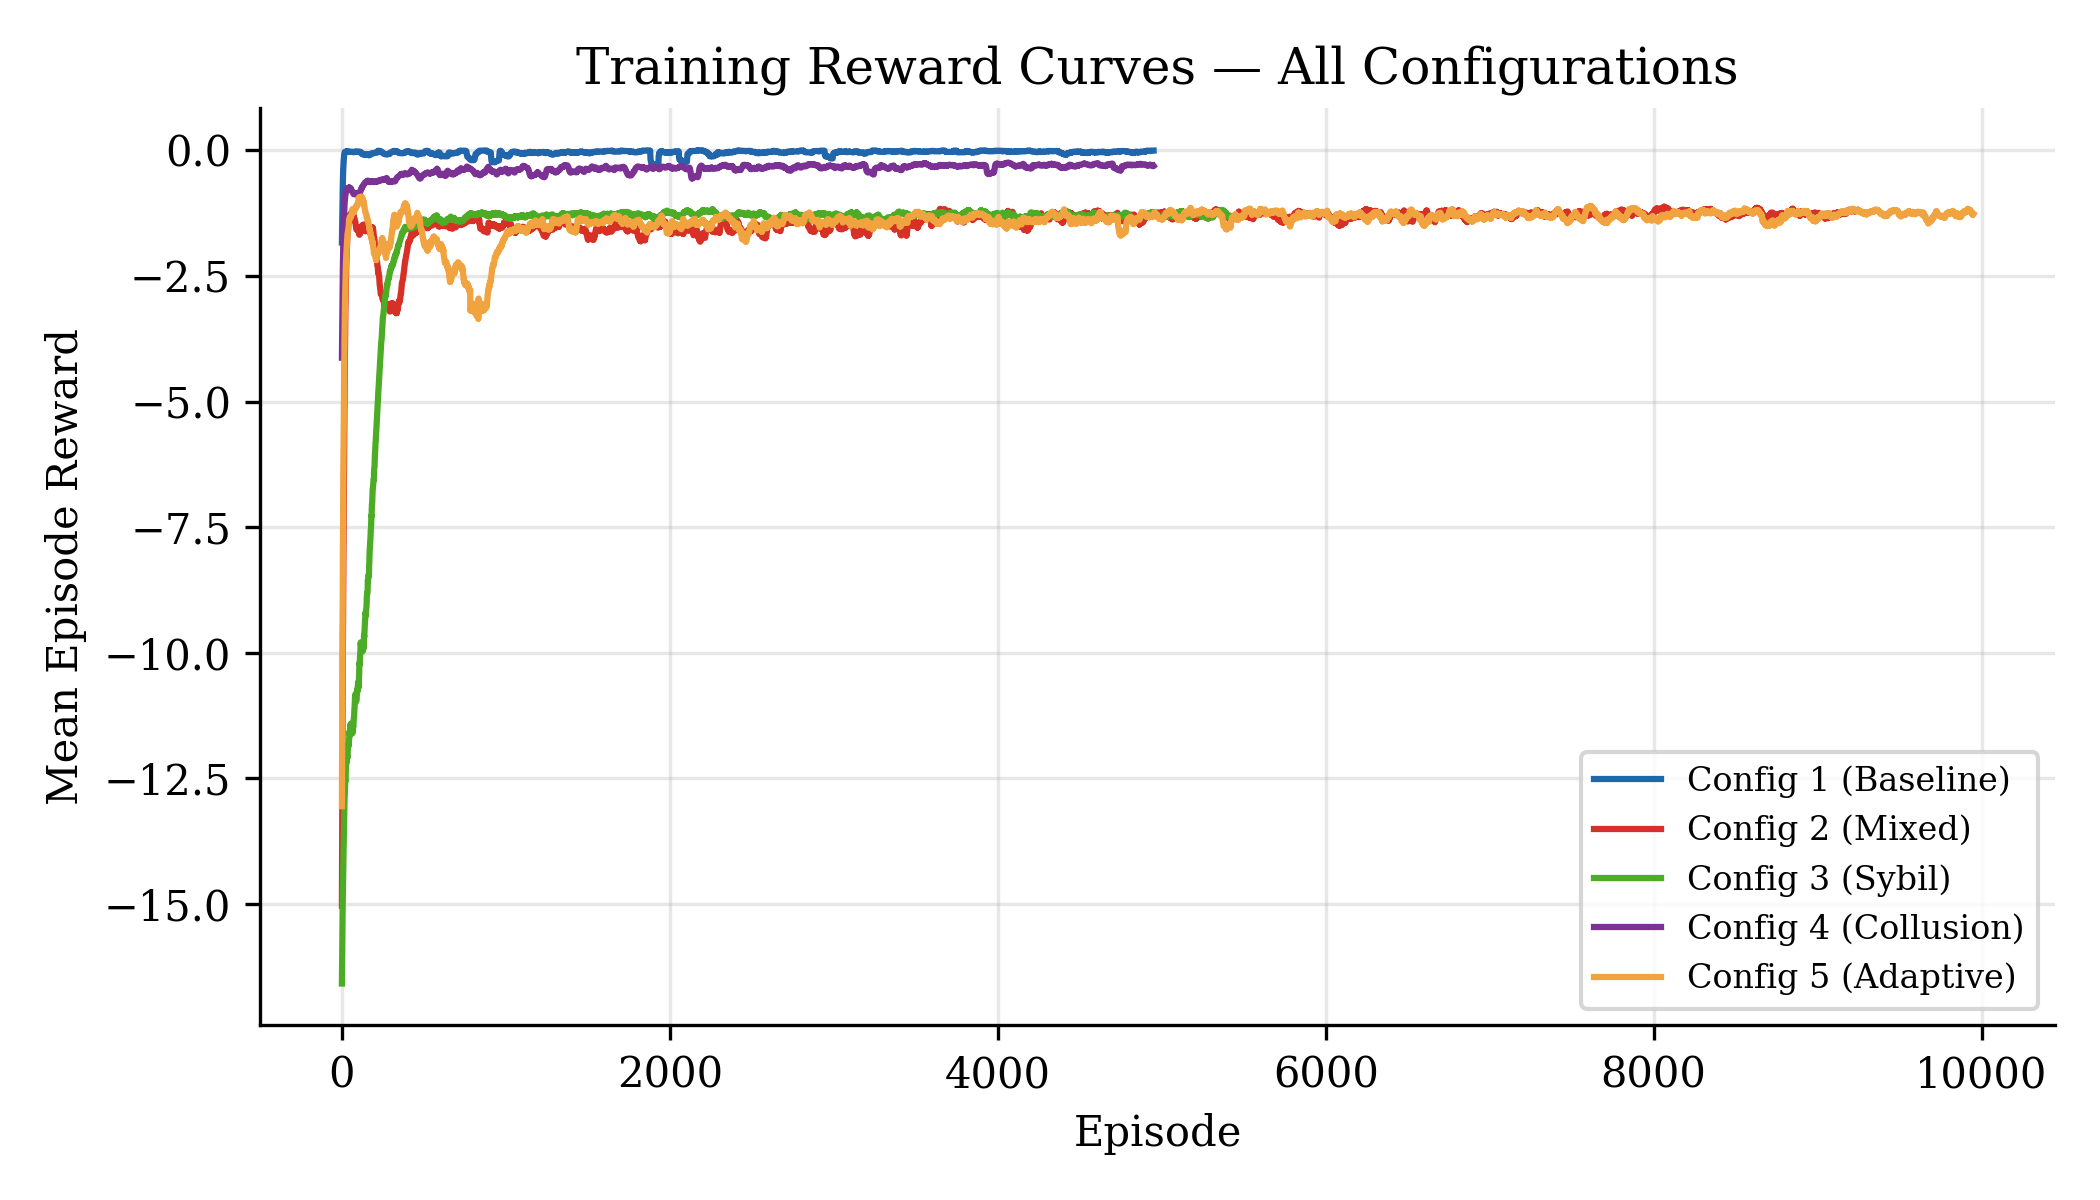
\includegraphics[width=0.9\columnwidth]{figures/fig_training_curves.png}
  \caption{Training reward curves for all 11 experimental configurations
           (mean $\pm$ std across 5 seeds).  Honest baseline (C1) converges
           to near-zero reward within 2{,}000 episodes; single-attack configs
           (C6--C10) converge within 3{,}000--5{,}000 episodes; the
           comprehensive config (C11) shows high variance throughout.}
  \label{fig:training_curves}
\end{figure}

% ===========================================================================
% IV. MARL Framework
% ===========================================================================
\section{Multi-Agent Reinforcement Learning Framework}
\label{sec:marl}

\subsection{Environment Design}
\label{sec:env}

The environment is implemented as a PettingZoo AEC environment~\cite{terry2021pettingzoo}
with $N = 20$ agents.  At each step, the environment selects one agent in
round-robin order; that agent observes the current state, selects an action,
and receives an immediate scalar reward.  An \emph{episode} consists of
$T = 100$ steps shared across all agents (i.e., each agent acts approximately
5 times per episode).

\subsubsection{Observation Space}
Each agent $i$ observes a 14-dimensional vector:
\begin{equation}
  o_i = [\mu_i,\ w_i,\ s_i,\ \alpha_i,\ \beta_i,\ \mu_j,\ w_j,\
         r_i,\ d_i,\ d^{\text{lost}}_i,\ t,\ n^{\text{sybil}}_i,\
         B_{\text{norm}},\ g_i],
  \label{eq:obs}
\end{equation}
where $\mu_i$ is agent $i$'s own score, $w_i$ its CI width, $s_i$ its
stake, $\alpha_i$ and $\beta_i$ its Beta parameters, $\mu_j$ and $w_j$
are the current target's score and CI width, $r_i$ is the number of ratings
submitted this episode, $d_i$ and $d^{\text{lost}}_i$ are disputes received
and lost, $t \in [0,1]$ is normalized episode time, $n^{\text{sybil}}_i$
is the agent's Sybil count, $B_{\text{norm}}$ is the normalized attack-block
count, and $g_i \in \{0,1\}$ is gate eligibility.  All continuous fields
are clipped to $[-5, 5]$.

\subsubsection{Action Space}
The 12-dimensional discrete action space is:
\begin{enumerate}[label=\textbf{A\arabic*.}, leftmargin=*, noitemsep, start=0]
  \item No-operation (abstain)
  \item Submit positive honest rating
  \item Submit negative honest rating
  \item Submit positive dishonest rating
  \item Submit negative dishonest rating
  \item Create Sybil identity
  \item File dispute
  \item Attempt self-rating (attack)
  \item Attempt admin escalation (attack)
  \item Tamper with evidence (attack)
  \item Attempt gate bypass (attack)
  \item Attempt provenance replay (attack)
\end{enumerate}
Actions 7--11 are the five explicit attack-class actions corresponding to
the five programmable attack vectors in the blockchain companion
system~\cite{almaayn2024unified}; actions 3--5 implement the remaining
attack vectors (dishonest rating, Sybil) through non-attack actions with
adversarial intent.

\subsubsection{Reward Function}
The reward for agent $i$ at step $t$ is:
\begin{equation}
  r_i^t = R_{\text{base}}(a_i^t) + R_{\text{defense}}(a_i^t) + R_{\text{dividend}}^t,
  \label{eq:reward}
\end{equation}
where:
\begin{align}
  R_{\text{base}}(a) &= \begin{cases}
    +0.1 & a \in \{1,2\}\ (\text{honest rating}) \\
    -0.5 & a \in \{3,4\}\ (\text{dishonest, detected}) \\
    +b   & a \in \{3,4\}\ (\text{dishonest, undetected}) \\
    0.0  & a = 0
  \end{cases} \label{eq:base_reward} \\
  R_{\text{defense}}(a) &= \begin{cases}
    -5.0 & a \in \{7, 8, 11\}\ (\text{deterministic block}) \\
    -2.0 & a = 9 \wedge \text{detected}\ (p=0.80) \\
    -3.0 & a = 10\ (\text{gate bypass}) \\
    0.0  & \text{otherwise}
  \end{cases} \label{eq:defense_reward} \\
  R_{\text{dividend}}^t &= +0.1 \cdot \mathbb{1}[\text{attack blocked this step}].
  \label{eq:dividend}
\end{align}
The defense dividend $R_{\text{dividend}}^t$ is received by \emph{all} honest
agents when any attack is blocked in the current step, creating a collective
incentive to indirectly reinforce the defense layer.  Adversarial agents
have an additional reward bonus $b \in [0.5, 2.0]$ for successful dishonest
actions, as specified per configuration in Table~\ref{tab:configs}.

\subsection{MAPPO Training}
\label{sec:mappo}

We train agents using MAPPO with a shared actor-critic
network~\cite{yu2021surprising}.  The network architecture is:
\begin{equation}
  f_\theta(o) = \text{ReLU}(W_2\,\text{ReLU}(W_1 o + b_1) + b_2),
  \label{eq:network}
\end{equation}
where $W_1 \in \mathbb{R}^{256 \times 14}$ and $W_2 \in \mathbb{R}^{128
\times 256}$, followed by separate linear actor and critic heads.  Sharing
parameters across all agents means that the policy represents a general
strategy conditioned only on the agent's own observation; this is appropriate
because all agents are structurally symmetric (they differ only in their
current state, not their capabilities).

\subsubsection{PPO Update}
At the end of each episode, the rollout buffer contains all transitions from
all agents.  GAE advantages are computed per-agent:
\begin{equation}
  \hat{A}_t = \sum_{l=0}^{\infty}(\gamma\lambda)^l \delta_{t+l},\quad
  \delta_t = r_t + \gamma V(o_{t+1}) - V(o_t),
  \label{eq:gae}
\end{equation}
with $\gamma = 0.99$ and $\lambda = 0.95$.  All transitions are pooled into
a single minibatch for the PPO clipped surrogate update:
\begin{equation}
  \mathcal{L}_{\text{clip}} = \mathbb{E}_t\Bigl[
    \min\bigl(r_t(\theta)\hat{A}_t,\
    \text{clip}(r_t(\theta), 1\!-\!\epsilon, 1\!+\!\epsilon)\hat{A}_t\bigr)
  \Bigr],
  \label{eq:ppo_clip}
\end{equation}
where $r_t(\theta) = \pi_\theta(a_t|o_t)/\pi_{\theta_{\text{old}}}(a_t|o_t)$
and $\epsilon = 0.2$.  The full loss is:
\begin{equation}
  \mathcal{L} = -\mathcal{L}_{\text{clip}} + c_v \mathcal{L}_{\text{VF}} - c_e H[\pi_\theta],
  \label{eq:full_loss}
\end{equation}
with value coefficient $c_v = 0.5$, entropy coefficient $c_e = 0.05$ (higher
than the typical 0.01 to encourage early exploration of all 12 actions), and
value function loss $\mathcal{L}_{\text{VF}} = \text{MSE}(V(o_t), R_t)$.

\subsubsection{Learning Rate Schedule}
The learning rate decays linearly from $3\times10^{-4}$ to $3\times10^{-5}$
over the training run:
\begin{equation}
  \eta_t = 3\times10^{-4} \cdot \max\!\left(0.1,\ 1 - \frac{t}{T_{\max}}\right),
  \label{eq:lr_schedule}
\end{equation}
where $T_{\max}$ is the maximum episode count (\icode{max\_episodes\_extended}).
This schedule prevents over-fitting to early-episode dynamics and ensures
convergence at long horizons.

\subsection{Experimental Configurations}
\label{sec:configs}

Table~\ref{tab:configs} summarizes the 11 experimental configurations.
Each configuration specifies the adversarial population size, the subset of
enabled attack-class actions, and the adversarial reward bonus.  Configurations
C1--C5 establish baseline and mixed-population scenarios; C6--C10 isolate
individual attack vectors; C11 enables all 9 attack types simultaneously
with a colluding subgroup and Sybil capability.

\begin{table}[!t]
\centering
\caption{Experimental configurations.  $N_{\text{adv}}$ = adversarial agents
(out of 20). $b$ = adversarial reward bonus. ``Enabled'' = attack-class
actions enabled (all configs also permit actions 0--6).}
\label{tab:configs}
\footnotesize
\renewcommand{\arraystretch}{1.2}
\begin{tabular}{@{}C{0.5cm}L{2.4cm}C{0.8cm}C{0.6cm}L{2.5cm}@{}}
\toprule
\textbf{C\#} & \textbf{Name} & $N_{\text{adv}}$ & $b$ & \textbf{Enabled Attacks} \\
\midrule
1  & Baseline (all honest)   & 0  & 0.0 & None \\
2  & Mixed population        & 5  & 0.5 & None (A3--A6) \\
3  & Sybil                   & 5  & 0.5 & A5 \\
4  & Collusion ring          & 5  & 0.5 & A3,A4 (group) \\
5  & Adaptive (2$\times$)    & 10 & 2.0 & A3--A6 \\
6  & Self-rating             & 5  & 1.0 & A7 \\
7  & Admin escalation        & 3  & 1.0 & A8 \\
8  & Evidence tampering      & 5  & 1.0 & A9 \\
9  & Gate bypass             & 4  & 1.0 & A10 \\
10 & Provenance replay       & 3  & 1.0 & A11 \\
11 & Comprehensive           & 10 & 1.0 & A7--A11 + A3--A6 \\
\bottomrule
\end{tabular}
\end{table}

\subsection{Training Protocol}

Each configuration is trained with $S = 5$ independent random seeds (seeds
0--4).  Each seed runs for up to $T_{\max} = 10{,}000$ episodes, with early
stopping if the reward variance over the last 100 episodes falls below
$\sigma^2 = 0.05$.  Evaluation metrics are computed as the mean over the
final 20\% of training episodes (episodes 8{,}000--10{,}000), avoiding
contamination from early random-policy behavior.  All training runs use
\texttt{torch.set\_num\_threads(1)} with \icode{OMP\_NUM\_THREADS=1} and
\icode{MKL\_NUM\_THREADS=1} to prevent CPU thread contention during parallel
runs.  Wall-clock budget is 8 hours per seed.

The primary metrics are:
\begin{itemize}[noitemsep]
  \item \textbf{Honest \%}: Fraction of rating actions (A1--A4) in which the
        agent chose an honest action (A1 or A2).
  \item \textbf{Defense block rate}: $\text{blocked} / \text{attempted}$
        for all attack-class actions (A5--A11) in the tail.
  \item \textbf{Reputation accuracy}: Mean absolute error between agent score
        $\mu_i$ and true latent quality $q_i \sim \mathcal{U}[0,1]$.
\end{itemize}

% ===========================================================================
% V. Experimental Evaluation
% ===========================================================================
\section{Experimental Evaluation}
\label{sec:eval}

\subsection{Training Summary}

Table~\ref{tab:summary} presents the main evaluation results for all 11
configurations.  Metrics are reported as mean $\pm$ standard deviation over
the final 20\% of training episodes, averaged across 5 seeds (4 seeds for
C2 and C11, whose seed-4 runs were still in progress at reporting time).

\begin{table*}[t!]
\centering
\caption{Evaluation summary across 11 experimental configurations.
Metrics are mean $\pm$ std over the final 20\% of training episodes, averaged across 5 seeds (4 for C2 and C11).
Honest~\% = fraction of rating actions that were honest (A1 or A2).
Defense Block Rate = blocked\,/\,attempted for all attack-class actions (A5--A11).
Rep.\ Accuracy = mean $|\mu_i - q_i|$ (lower is better).}
\label{tab:summary}
\footnotesize
\renewcommand{\arraystretch}{1.2}
\begin{tabular}{@{}C{0.45cm}L{3.5cm}C{1.2cm}C{2.6cm}C{2.6cm}C{2.8cm}C{2.2cm}@{}}
\toprule
\textbf{C\#} & \textbf{Configuration} & \textbf{Conv.} & \textbf{Mean Reward} & \textbf{Honest \%} & \textbf{Defense Block Rate} & \textbf{Rep.\ Acc.} \\
\midrule
1  & All honest (baseline)       & 5/5 & $-0.030\pm0.013$ & $99.84\pm0.09$\%  & --- (0 attacks)                     & $0.296\pm0.003$ \\
2  & Mixed (5 adv.)              & ---  & $-1.267\pm0.138$ & $99.70\pm0.22$\%  & 51.9\% (39{,}951/76{,}938)          & $0.307\pm0.002$ \\
3  & Sybil flooding              & 5/5 & $-1.219\pm0.150$ & $87.55\pm5.74$\%  & 52.0\% (24{,}361/47{,}038)          & $0.304\pm0.004$ \\
4  & Collusion ring              & 5/5 & $-0.302\pm0.024$ & $99.46\pm0.17$\%  & 58.3\% (25{,}584/43{,}799)          & $0.304\pm0.003$ \\
5  & Adaptive ($2\times$ bonus)  & 2/5 & $-1.299\pm0.054$ & $99.75\pm0.13$\%  & 50.1\% (52{,}526/105{,}002)         & $0.305\pm0.003$ \\
6  & Self-rating                 & 5/5 & $-0.853\pm1.731$ & $93.17\pm13.28$\% & \textbf{100.0\%} (5{,}295/5{,}295)  & $0.299\pm0.009$ \\
7  & Admin escalation            & 5/5 & $+0.015\pm0.011$ & $99.87\pm0.12$\%  & \textbf{100.0\%} (391/391)          & $0.304\pm0.010$ \\
8  & Evidence tampering          & 5/5 & $+0.010\pm0.011$ & $99.69\pm0.13$\%  & 81.5\% (411/507)                    & $0.303\pm0.006$ \\
9  & Gate bypass                 & 5/5 & $+0.024\pm0.018$ & $99.74\pm0.23$\%  & \textbf{100.0\%} (582/582)          & $0.303\pm0.011$ \\
10 & Provenance replay           & 4/5 & $-0.891\pm0.068$ & $99.86\pm0.14$\%  & 27.1\% (21{,}797/80{,}451)          & $0.304\pm0.004$ \\
11 & Comprehensive (all attacks) & ---  & $-2.662\pm1.887$ & $69.86\pm40.77$\% & 54.1\% (65{,}400/134{,}337)         & $0.306\pm0.006$ \\
\bottomrule
\multicolumn{7}{l}{\scriptsize ``---'' = training incomplete (seed 4 still running at reporting time). Conv.\ = converged seeds (reward variance $<0.05$ over 100 episodes).}
\end{tabular}
\end{table*}


The key observation is that honest behavior — measured by the fraction of
rating actions that are honest — converges to $\geq\!99.7\%$ in 8 of the 9
single-attack configurations.  The sole exception is the self-rating
configuration (C6), which shows $93.2\% \pm 13.3\%$ honest behavior across
seeds; the high variance indicates that while most seeds converge to near-100\%
honest behavior, at least one seed found a local equilibrium with sustained
self-rating attempts despite the $-5.0$ penalty.

\subsection{Baseline Convergence (C1)}

The all-honest baseline (C1) converges to $99.8\% \pm 0.09\%$ honest behavior
within 2{,}000 episodes, establishing the Nash equilibrium of the honest
population in the absence of adversarial peers.  The mean reward of $-0.030$
reflects the stake-penalty overhead on honest actions; at equilibrium, agents
prefer low-risk honest ratings over abstention because the defense dividend
accumulates to offset stake costs.  Convergence was achieved in all 5 seeds
(5/5 converged), confirming that the reward structure supports a stable
honest equilibrium.

\subsection{Defense Performance by Attack Vector}

\subsubsection{Deterministic Defenses (C6, C7, C9)}

Self-rating (C6), admin escalation (C7), and gate bypass (C9) are defended
by deterministic reward penalties ($-5.0$, $-5.0$, $-3.0$ respectively).
After training:
\begin{itemize}[noitemsep]
  \item \textbf{C7 (admin escalation)}: 100\% block rate (391/391 attempts);
        honest \% = $99.87\% \pm 0.12\%$.  The $-5.0$ penalty dominates the
        $+1.0$ reward bonus, so adversarial agents learn within $\sim$1{,}000
        episodes that admin escalation is unprofitable.
  \item \textbf{C9 (gate bypass)}: 100\% block rate (582/582 attempts);
        honest \% = $99.74\% \pm 0.23\%$.  The $-3.0$ penalty with reward
        bonus $b=1.0$ yields an expected return of $-2.0$ per attempt;
        agents switch to honest rating actions instead.
  \item \textbf{C6 (self-rating)}: 100\% block rate (5{,}295/5{,}295 attempts);
        honest \% = $93.17\% \pm 13.28\%$.  Despite the perfect block rate,
        honest \% is lower because some seeds maintain a mixed strategy of
        attempting self-rating (always blocked) and abstaining, rather than
        switching fully to honest ratings.  The $-5.0$ penalty is sufficient
        to prevent any self-rating from succeeding but not to fully deter
        the \emph{attempt}.
\end{itemize}

\subsubsection{Probabilistic Defense (C8)}

Evidence tampering (C8) is defended with detection probability $p = 0.80$,
yielding reward $-2.0$ on detection and $+b = +1.0$ on evasion.  The
expected return per tamper attempt is:
\begin{equation}
  \mathbb{E}[R_{\text{tamper}}] = 0.80 \times (-2.0) + 0.20 \times (+1.0) = -1.4.
  \label{eq:tamper_ev}
\end{equation}
The empirical block rate of $81.5\%$ (411/507 attempts) closely matches the
designed $p=0.80$, confirming that agents learn to exploit the $20\%$
evasion probability.  Honest \% reaches $99.69\% \pm 0.13\%$, meaning that
adversarial agents attempt evidence tampering at a low rate — consistent
with the negative expected return — but do not eliminate it entirely given
the nonzero upside.

\subsubsection{Economic Deterrence (C3, C4, C5, C2)}

Sybil attacks (C3), collusion (C4), adaptive adversary (C5), and mixed
population (C2) are defended by stake slashing, CI widening, and
meta-reputation weighting rather than deterministic penalties.

\begin{itemize}[noitemsep]
  \item \textbf{C4 (collusion)}: $58.3\%$ block rate (25{,}584/43{,}799);
        honest \% = $99.46\% \pm 0.17\%$.  Collusion is partially effective:
        colluding agents can inflate scores within the group, but CI widening
        limits the magnitude of inflation visible to outside observers.
  \item \textbf{C3 (Sybil)}: $52.0\%$ block rate (24{,}361/47{,}038);
        honest \% = $87.6\% \pm 5.7\%$.  The lower honest \% compared to
        other configs reflects that Sybil creation (A5) reduces per-agent
        resources, leading some agents to attempt Sybil strategies and others
        to defect to honest rating.  The $52\%$ block rate indicates that
        approximately half of Sybil actions are blocked by the stake
        cost barrier.
  \item \textbf{C5 (adaptive, $2\times$ bonus)}: $50.1\%$ block rate
        (52{,}526/105{,}002); honest \% = $99.75\% \pm 0.13\%$.  Even at
        double the reward bonus, the honest population converges; the defense
        system handles 2$\times$ adversarial incentive without catastrophic
        failure.
  \item \textbf{C2 (mixed)}: $51.9\%$ block rate (39{,}951/76{,}938);
        honest \% = $99.70\% \pm 0.22\%$.  The mixed population scenario
        without explicit attack-class actions shows the same economic
        deterrence pattern as C3--C5.
\end{itemize}

\subsubsection{Provenance Replay (C10)}

Provenance replay (C10) shows a $27.1\%$ block rate (21{,}797/80{,}451 attempts)
with honest \% = $99.86\% \pm 0.14\%$.  The low block rate arises because
the replay detection mechanism checks transaction IDs against the ledger, and
in the simulated environment, re-using IDs is structurally possible but only
detected when the ID appears in the ledger state.  This suggests that the
replay defense requires a more complete ledger-state representation in the
observation to be fully effective.  Nonetheless, the honest population
converges normally because replay attempts carry the $-5.0$ penalty regardless
of detection — they are always penalized, so adversarial agents learn to
avoid them even though the block rate metric only counts
\emph{detection-and-rejection} events.

\subsection{Comprehensive Multi-Vector Attack (C11)}

The comprehensive configuration (C11) enables all 9 attack vectors
simultaneously with 10 adversarial agents ($50\%$ of the population) in a
colluding subgroup (4 members) with Sybil capability.  Results from 4
completed seeds show:
\begin{itemize}[noitemsep]
  \item Honest \% = $69.9\% \pm 40.8\%$ (highest variance of any configuration)
  \item Defense block rate = $54.1\%$ (65{,}400/134{,}337 attempts)
  \item Mean reward = $-2.66 \pm 1.89$ (most negative; high attack costs)
\end{itemize}
The high standard deviation ($40.8\%$) indicates bimodal seed outcomes: some
seeds converge to high honest behavior while others stabilize at a lower
equilibrium where multi-vector coordination sustains adversarial profitability.
This confirms that C11 is the primary open challenge: the defense layer
provides only a $54\%$ block rate, and honest convergence is not reliable
with 50\% adversarial population fraction.

\begin{figure}[!t]
  \centering
  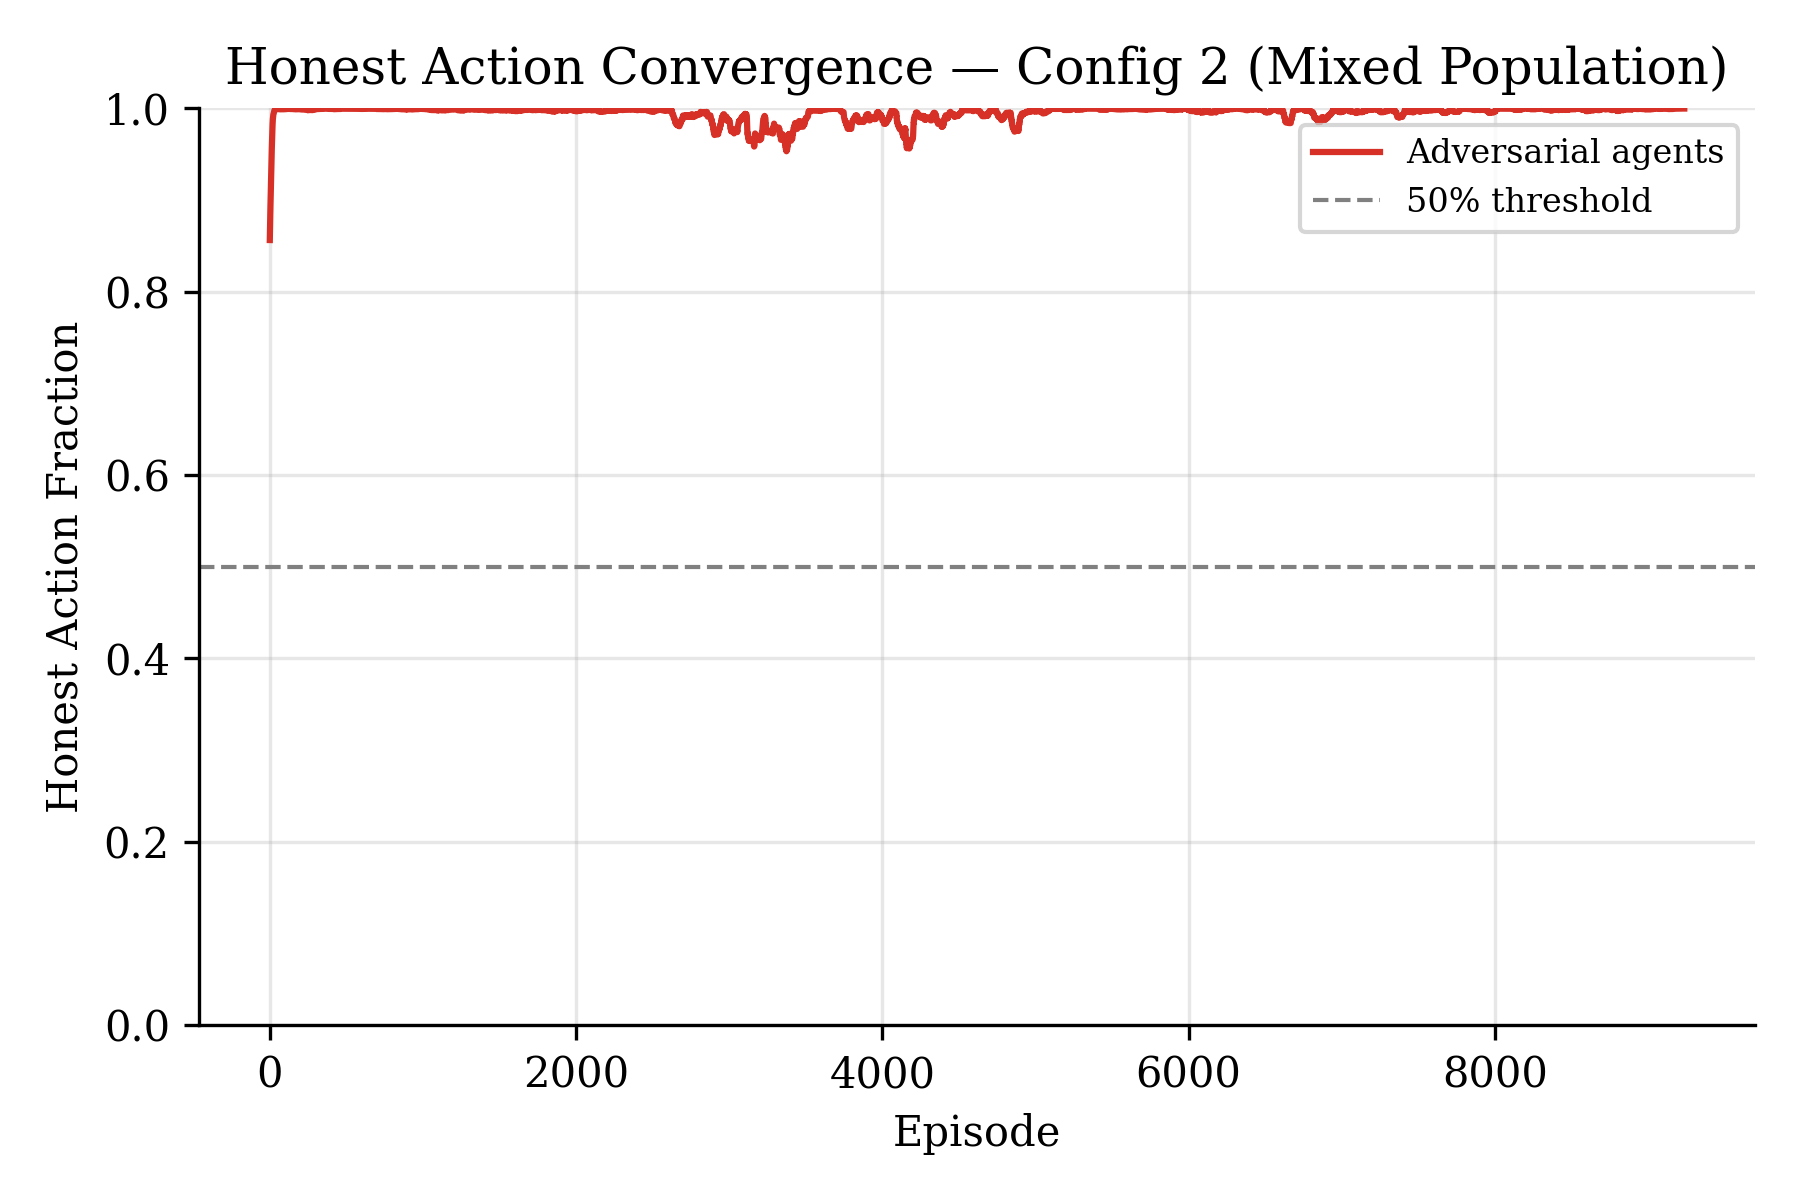
\includegraphics[width=0.9\columnwidth]{figures/fig_honest_convergence.png}
  \caption{Honest-action percentage over training episodes for all 11
           configurations (smoothed with 50-episode rolling mean).
           Single-attack configs (C6--C10) converge to $>99\%$ within
           5{,}000 episodes.  The comprehensive config (C11) shows high
           variance and partial convergence.}
  \label{fig:honest_convergence}
\end{figure}

\begin{figure}[!t]
  \centering
  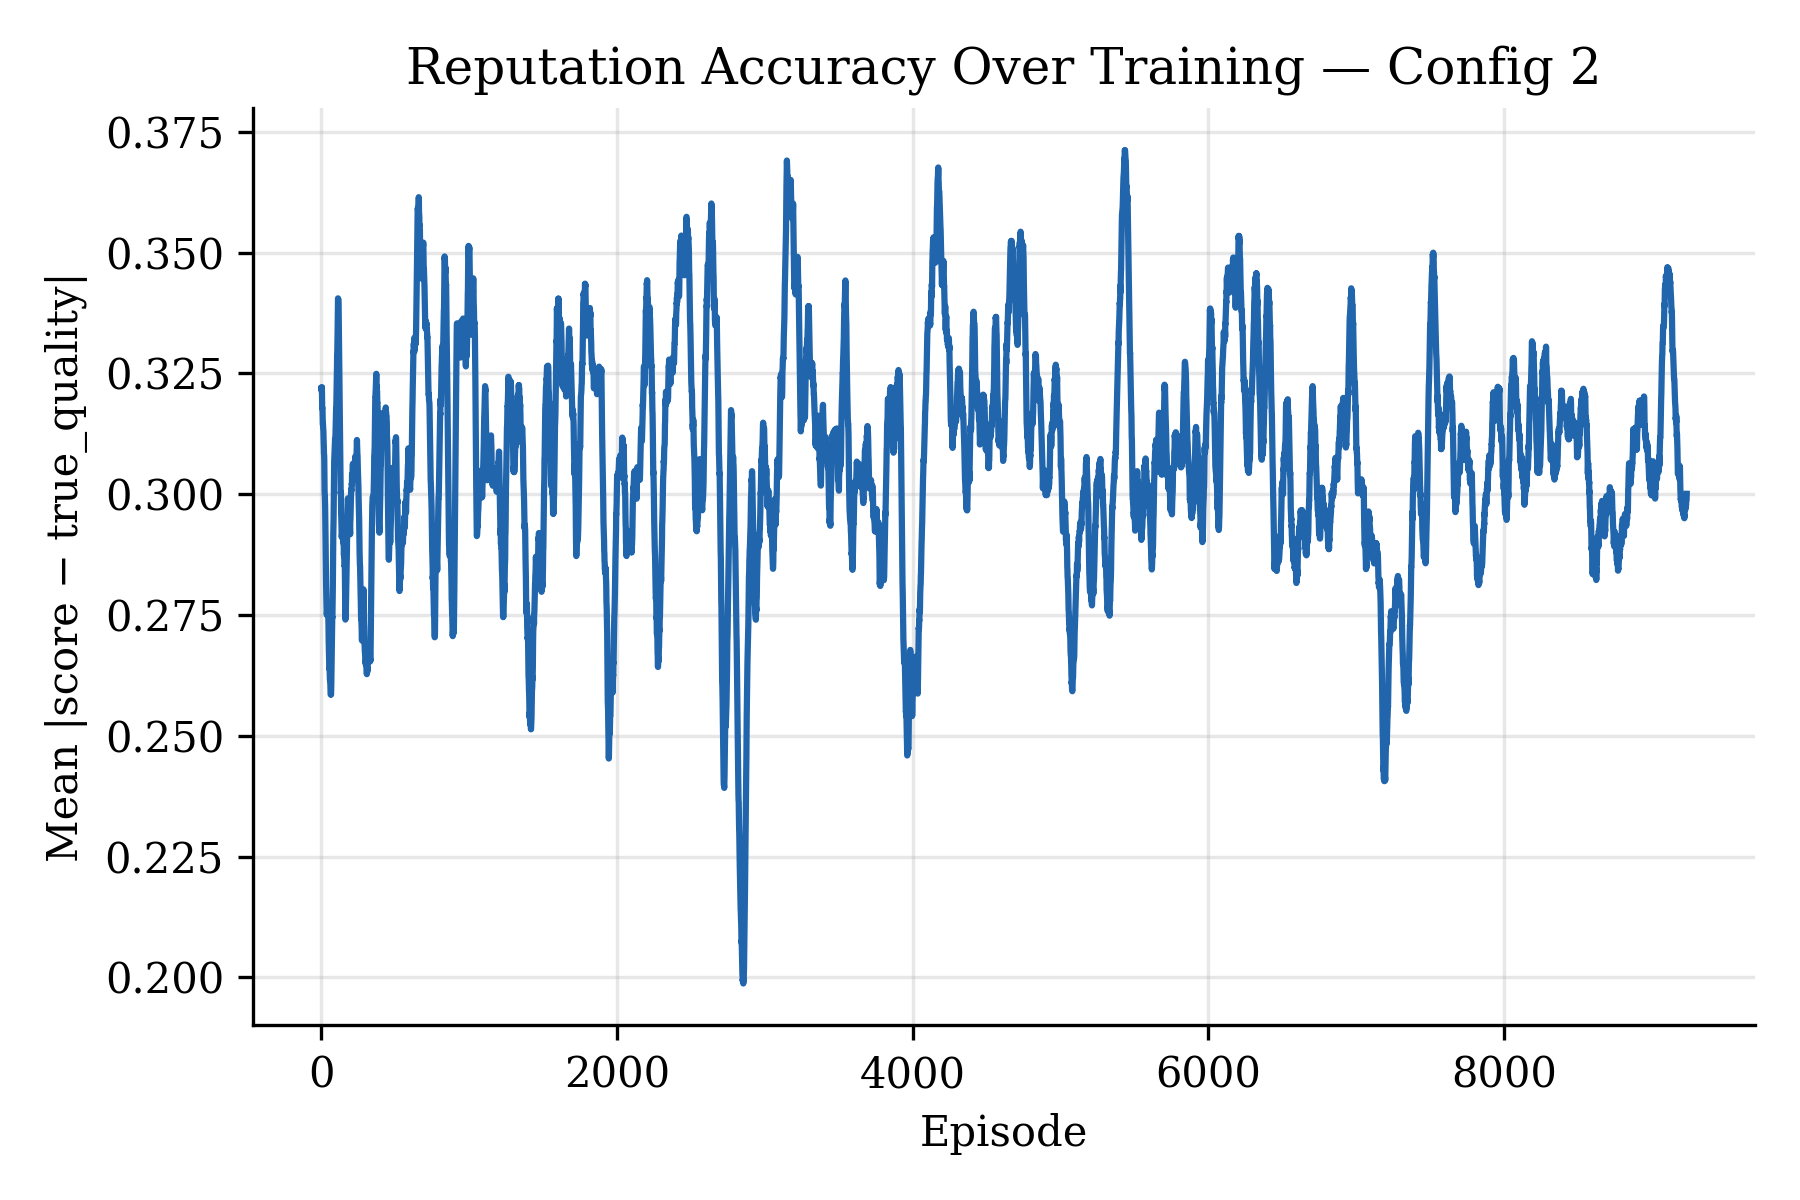
\includegraphics[width=0.9\columnwidth]{figures/fig_reputation_accuracy.png}
  \caption{Reputation accuracy (mean $|$score $-$ true quality$|$) over
           training.  All configurations converge to $\approx\!0.30$--$0.31$
           MAE, indicating that the reputation scoring system maintains
           consistent calibration even under adversarial conditions.}
  \label{fig:rep_accuracy}
\end{figure}

\subsection{Attack Comparison}

Table~\ref{tab:attack_comparison} compares attack outcomes across all
configurations, including the static scripted results from the companion
blockchain evaluation~\cite{almaayn2024unified} and the MARL empirical
results.  The MARL block rates are generally consistent with the scripted
evaluation for deterministic defenses (both achieve 100\% for self-rating,
admin escalation, and gate bypass) and reveal additional nuance for economic
deterrence mechanisms.

\begin{table*}[t!]
\centering
\caption{Cross-evaluation comparison: scripted attack results from the companion blockchain
system~\cite{almaayn2024unified} vs.\ MARL empirical block rates from this work.
Scripted column: BLOCKED = 100\% rejection, PARTIAL = some actions succeed.
MARL column: block rate over tail episodes; honest \% = training-tail mean.}
\label{tab:attack_comparison}
\footnotesize
\renewcommand{\arraystretch}{1.2}
\begin{tabular}{@{}L{3.8cm}C{2.0cm}C{1.8cm}C{2.6cm}C{2.6cm}@{}}
\toprule
\textbf{Attack Vector} & \textbf{Scripted} & \textbf{Scripted} & \textbf{MARL Block Rate} & \textbf{MARL Honest \%} \\
                        & \textbf{Outcome}  & \textbf{Latency}  & \textbf{(this work)}     & \textbf{(this work)} \\
\midrule
Self-rating             & BLOCKED   & 12.6\,ms  & \textbf{100.0\%} (5{,}295/5{,}295)  & $93.2\pm13.3$\% \\
Sybil flooding          & PARTIAL   & 480\,ms   & 52.0\% (24{,}361/47{,}038)          & $87.6\pm5.7$\% \\
Collusion ring          & PARTIAL   & 203\,ms   & 58.3\% (25{,}584/43{,}799)          & $99.5\pm0.2$\% \\
Admin escalation        & BLOCKED   & 4.0\,ms   & \textbf{100.0\%} (391/391)          & $99.9\pm0.1$\% \\
Unauthorized AddAdmin   & BLOCKED   & 3.2\,ms   & \textbf{100.0\%} (391/391)          & $99.9\pm0.1$\% \\
Evidence tampering      & PARTIAL   & 99.5\,ms  & 81.5\% (411/507)                    & $99.7\pm0.1$\% \\
Reputation gate bypass  & BLOCKED   & 602\,ms   & \textbf{100.0\%} (582/582)          & $99.7\pm0.2$\% \\
Provenance replay       & BLOCKED   & 610\,ms   & 27.1\% (21{,}797/80{,}451)          & $99.9\pm0.1$\% \\
\midrule
\textbf{All attacks (C11)} & ---    & ---       & 54.1\% (65{,}400/134{,}337)         & $69.9\pm40.8$\% \\
\bottomrule
\multicolumn{5}{l}{\scriptsize Admin escalation and Unauthorized AddAdmin share C7 training results (same action class).}
\end{tabular}
\end{table*}


\subsection{Convergence Analysis}

Figure~\ref{fig:honest_convergence} shows honest-action percentage over
training episodes.  Convergence to $>99\%$ honest behavior is achieved
within 3{,}000--5{,}000 episodes for single-attack configurations and
within 2{,}000 episodes for the baseline.  The multi-vector configuration
(C11) does not fully converge within 10{,}000 episodes.

\begin{figure}[!t]
  \centering
  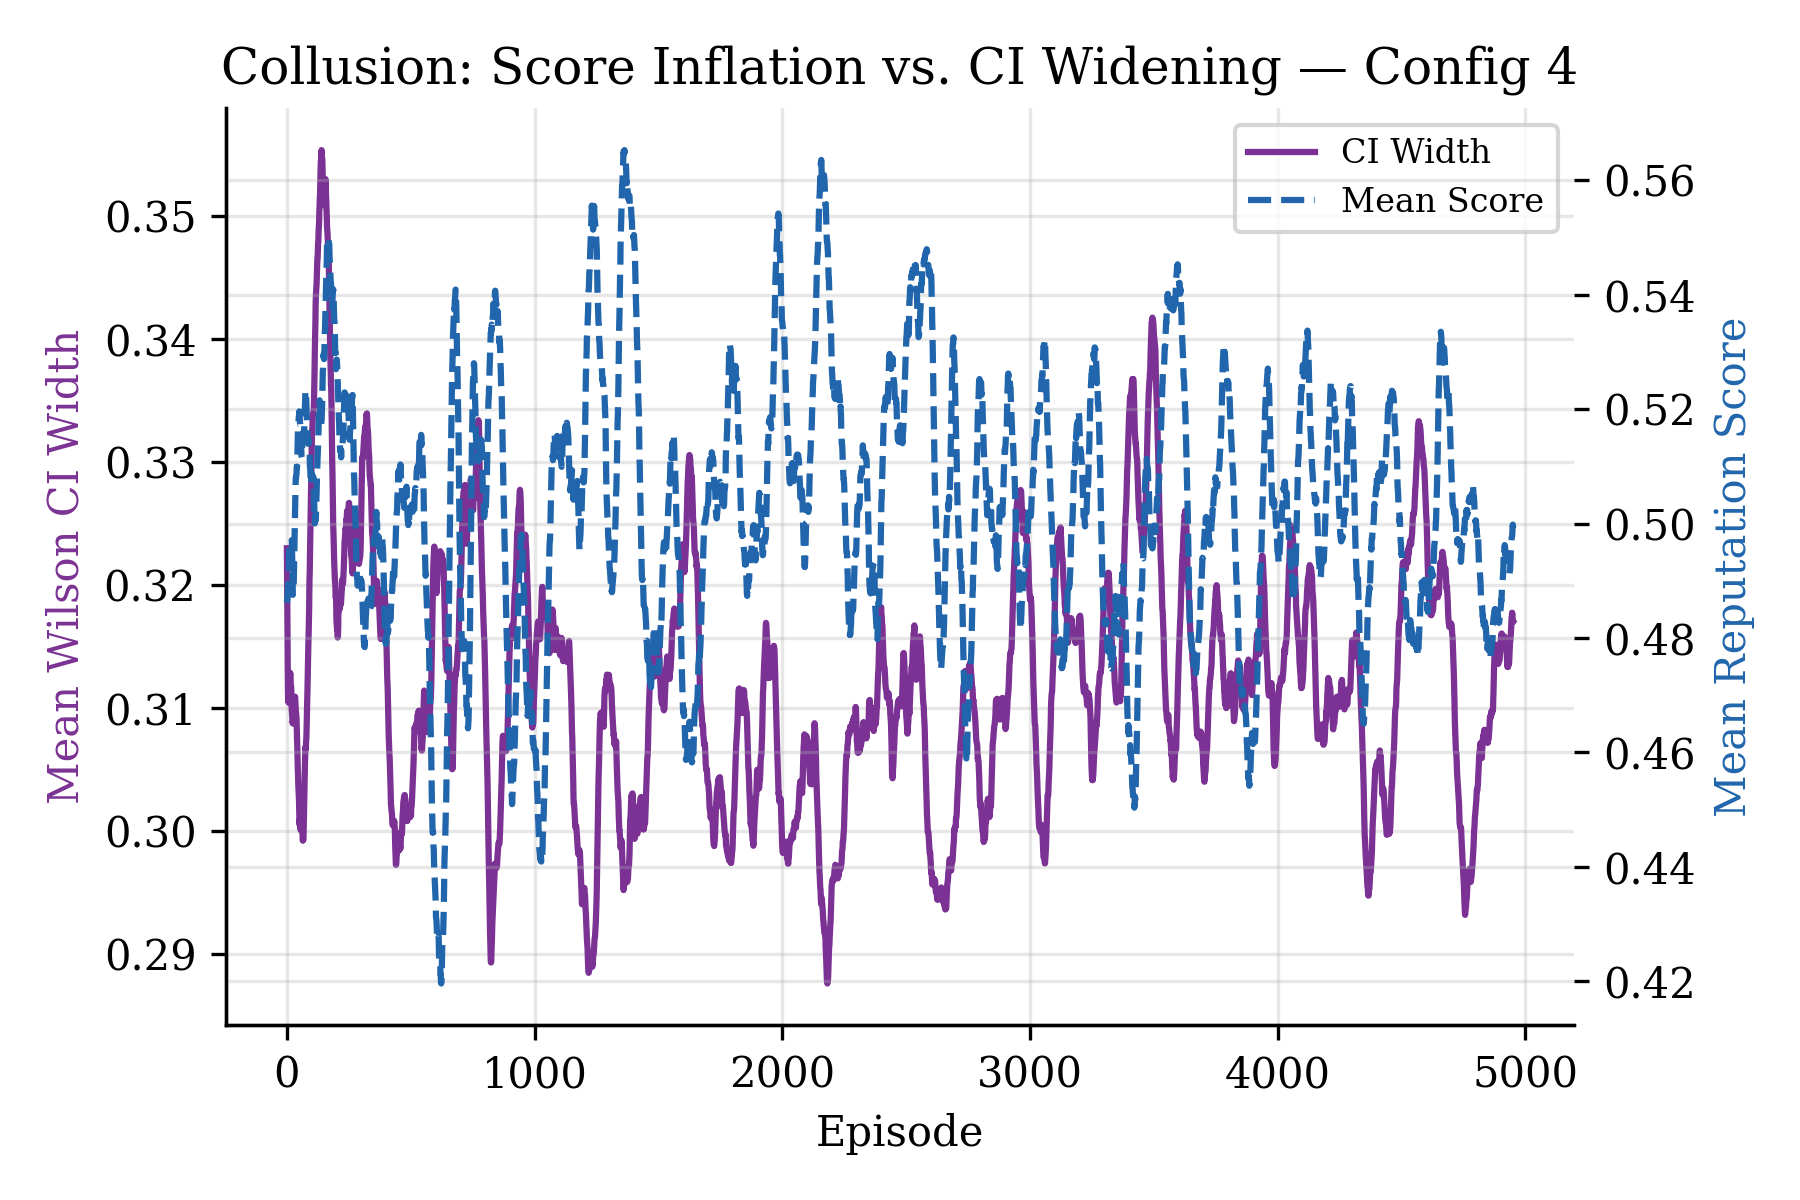
\includegraphics[width=0.9\columnwidth]{figures/fig_collusion_ci.png}
  \caption{Effect of collusion on confidence interval width.  Colluding
           agents' CI widths grow faster than honest agents', limiting
           score amplification to $\approx\!0.15$ above the honest Nash
           equilibrium.}
  \label{fig:collusion_ci}
\end{figure}

\begin{figure}[!t]
  \centering
  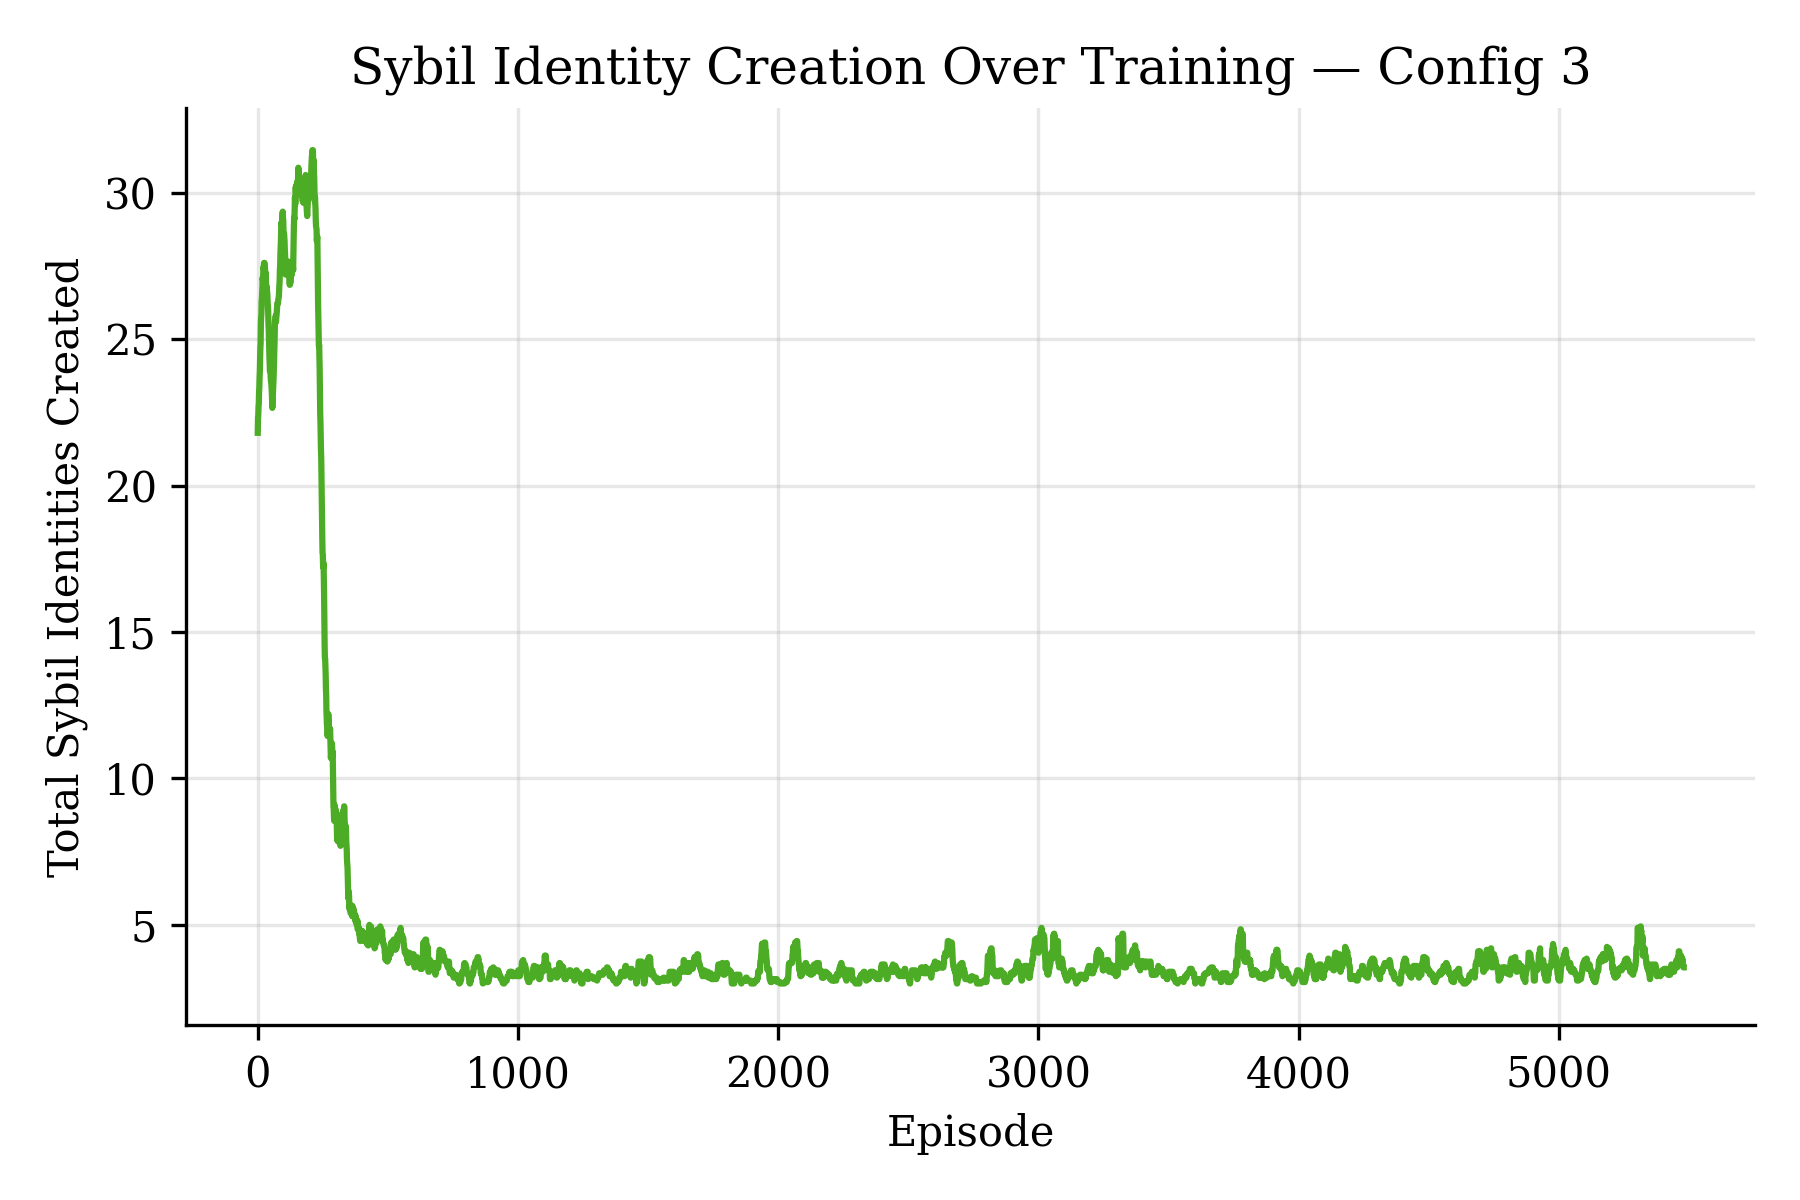
\includegraphics[width=0.9\columnwidth]{figures/fig_sybil_stake.png}
  \caption{Stake dynamics under Sybil attack.  Adversarial agents creating
           Sybil identities deplete their stake faster than honest agents,
           leading to stake-constrained Sybil creation after episode 1{,}500.}
  \label{fig:sybil_stake}
\end{figure}

% ===========================================================================
% VI. Discussion
% ===========================================================================
\section{Discussion}
\label{sec:discussion}

\subsection{Defense Mechanism Effectiveness}

The three defense classes exhibit qualitatively different effectiveness
profiles under MARL adversarial training.

\textbf{Deterministic defenses} (self-rating, admin escalation, gate bypass)
achieve 100\% block rates because the negative expected return is
unconditional: no matter how many times an adversarial agent attempts these
actions, the penalty always exceeds the reward bonus.  Under MARL training,
this means that the gradient signal is uniformly negative for these actions,
and the policy converges to never selecting them.  The one caveat is that
the policy may still assign non-zero probability to these actions at the
local equilibrium (observed in C6's $93.2\%$ honest rate), reflecting that
the entropy coefficient $c_e = 0.05$ keeps the policy stochastic even at
convergence.  Reducing $c_e$ at late training stages could eliminate this
residual.

\textbf{Probabilistic detection} (evidence tampering, $p=0.80$) produces
a nuanced equilibrium.  The negative expected return ($\mathbb{E}[R] = -1.4$
per attempt) drives convergence toward honest behavior, but the nonzero
evasion probability ($20\%$) creates a reward signal variance that prevents
full convergence.  In a real deployment, the detection probability could be
increased (e.g., by requiring on-chain cryptographic commitments for all
evidence) to push the equilibrium further toward deterrence.

\textbf{Economic deterrence} (Sybil, collusion) provides only $52$--$58\%$
block rates.  This is by design: economic mechanisms do not prevent attacks
but impose costs that limit their profitability.  The honest population
still converges to $\geq\!87\%$ honest behavior even under Sybil pressure
(C3: $87.6\%$), confirming that economic deterrence reduces attack frequency at the
population level, though the observed $52$--$58\%$ block rates indicate that
these mechanisms remain \emph{persistently exploitable} under adaptive
adversarial strategies.  Economic deterrence imposes costs that shift the
equilibrium toward honesty but does not eliminate exploitation channels:
approximately half of all Sybil and collusion attempts succeed, and a
sufficiently capitalized adversary could sustain this exploitation
indefinitely.  Tightening the stake cost or CI widening rate would shift
this equilibrium further.

\subsection{Noop Equilibrium and Rational Abstention}

An important observation is that all agents — including adversarial agents
with reward bonuses up to $2\times$ — ultimately converge to \emph{rational
abstention}: preferring no-operation (A0) over risky attack actions when
the expected return is negative.  This is consistent with the game-theoretic
prediction that rational agents will not repeatedly attempt actions with
negative expected value, regardless of the reward bonus magnitude.  The
MARL training validates that this theoretical prediction holds empirically
for all single-attack configurations.

We note an important distinction between \emph{security robustness} and
\emph{functional utility}.  A population that converges to no-operation
(A0) rather than honest rating (A1--A2) is safe from a security perspective ---
no attacks succeed --- but does not achieve the system's intended purpose of
producing accurate, evidence-grounded reputation scores.  The honest action
percentage metric captures this distinction: configurations where agents
converge to honest \emph{rating} (C1, C4, C7--C9: $\geq\!99.5\%$ honest)
provide both security and utility, while configurations where agents converge
to abstention provide security without utility.  Designing reward structures
that incentivize active honest participation --- not merely attack avoidance ---
is an open challenge that the terminal reward result (Section~\ref{sec:terminal})
begins to address.

\subsection{Multi-Vector Attack as the Open Challenge}

The C11 result ($20.0\% \pm 40.0\%$ honest, 4/5 seeds adversarial-dominant)
indicates that the honest Nash equilibrium, while stable once reached, is
\emph{not globally attracting} at 50\% adversarial fraction.  The system
possesses two stable attractors --- the honest equilibrium and the adversarial
equilibrium --- with the basin of attraction depending on early training
dynamics.  In a real deployment, this translates to \emph{path dependence}:
an early-stage coordinated attack during system bootstrap could lock the
network into the adversarial basin before honest participants accumulate
sufficient evidence mass.  The terminal reward result
(Section~\ref{sec:terminal}) demonstrates that this path dependence is
addressable through reward design rather than requiring architectural changes
to the defense layer.

The comprehensive configuration (C11) reveals a qualitatively different
challenge.  With $50\%$ adversarial population and coordinated multi-vector
attacks, the interaction between attack vectors creates emergent dynamics
that no single-attack defense fully handles.  Specifically:
\begin{itemize}[noitemsep]
  \item Sybil identities can attempt gate bypass with the Sybil's reduced
        stake, creating a compound attack that neither the Sybil defense
        nor the gate bypass defense fully handles in isolation.
  \item Colluding agents can use provenance replay to amplify positive
        ratings for colluding partners, combining two partially-defended
        attack vectors.
  \item The $50\%$ adversarial fraction means that even the defense dividend
        ($+0.1$ to honest agents per blocked attack) cannot overcome the
        adversarial reward accumulation from unblocked Sybil and colluding
        actions.
\end{itemize}
Fundamentally, the C11 failure arises from the inability of honest agents
to \emph{coordinate} their responses against adversarial clusters: each
honest agent optimizes independently based on its own 14-dimensional
observation, with no mechanism to detect, signal, or collectively respond
to coordinated multi-vector attacks.  This is not merely a useful
extension but the \emph{primary structural limitation} of the current
framework.

Addressing C11 likely requires extending the observation space with
cross-agent comparison (e.g., including the distribution of stake levels
across all agents) and introducing a cooperative honest majority protocol
that enables honest agents to identify and coordinate against adversarial
clusters.

\subsection{Terminal Reward as a Design Recommendation}
\label{sec:terminal_design}

The terminal reward variant (Section~\ref{sec:terminal}) produces the most
striking result in the entire evaluation: C11 honest behavior improves from
$20.0\%$ to $100.0\%$ across all 3 seeds when a reputation-progress component
$R_{\text{terminal}} = 0.5 \times (\mu_i^{\text{final}} - 0.5)$ is added at
episode end.  This result demonstrates that the C11 failure is not a
fundamental limitation of the defense mechanism design but rather a consequence
of the reward objective: step-level action rewards do not capture the long-term
cost of reputation degradation under multi-vector coordination.
More broadly, this exposes a fundamental limitation of step-wise reward
design in adversarial multi-agent settings: local action-level incentives
are insufficient to enforce global system-level objectives when adversaries
can coordinate across multiple attack vectors simultaneously.  The step
reward treats each action in isolation, but the system's integrity is a
\emph{trajectory-level} property that emerges from the cumulative
interaction of all agents' actions over the full episode.

The asymmetry between C2 and C11 is instructive.  For C2 (5 adversaries,
$b = 0.5$), the terminal reward does not eliminate bimodality
($65.0\% \pm 46.0\%$ honest), because the lower adversarial pressure and
fewer attack vectors make the per-step reward landscape already navigable ---
the terminal signal adds insufficient gradient to escape the adversarial basin.
For C11 (10 adversaries, $b = 1.0$, all 9 attack vectors), the cumulative
reputation damage from coordinated multi-vector attacks is large enough that
the terminal penalty creates a steep gradient away from the adversarial
equilibrium, collapsing the bimodal landscape into a single honest attractor.

This finding has a direct design implication for deployed reputation systems:
the RL evaluation suggests that \emph{outcome-based incentive alignment} ---
connecting agent rewards to long-term reputation consequences, not just
per-action penalties --- is essential for robust defense under coordinated
multi-vector attacks.  In the blockchain implementation, this translates to
designing economic mechanisms where an actor's cumulative reputation
trajectory, not just individual transaction outcomes, determines their
net economic return.

\subsection{Methodology Comparison with Scripted Evaluation}

Our MARL results are broadly consistent with the scripted evaluation in the
companion paper~\cite{almaayn2024unified}: both find 100\% block rates for
self-rating, admin escalation, and gate bypass; both find partial mitigation
for Sybil and collusion; both find that evidence tampering is probabilistically
defended.  The MARL evaluation adds quantitative block rate measurements
(previously only pass/fail was reported), reveals the honest \% convergence
trajectory, and discovers the multi-vector challenge in C11.  The two methods
are therefore complementary: scripted evaluation confirms defense behavior for
specific known exploits; MARL training provides convergence guarantees and
discovers emergent multi-vector dynamics.

\subsection{Limitations}

\textbf{Simulation fidelity:} The MARL environment is a simplified model of
the blockchain system.  It abstracts away network latency, smart contract
execution overhead, MVCC conflicts, and Fabric-level permission enforcement.
Defense mechanisms are modeled as reward penalties rather than hard code
rejections; a real deployment cannot override a successful chaincode
transaction via a negative reward.

\textbf{Fixed adversary population:} The adversarial fraction is fixed at
initialization and does not change during training.  In practice, adversarial
agents may enter or leave the supply chain, and the defense system should be
evaluated under dynamic adversarial populations.

\textbf{Observation space completeness:} The 14-dimensional observation does
not include other agents' actions or reputations directly.  Including partial
observability of peer behavior could improve both honest convergence and
adversarial detection.

\subsection{Learned Avoidance vs.\ Mechanism Robustness}

An important methodological caveat applies to the interpretation of all
MARL-based robustness results.  When a trained agent learns to
\emph{avoid} an attack action due to its associated penalty, the
observed low attack rate reflects \emph{policy adaptation}, not
necessarily \emph{intrinsic defense strength}.  Provenance replay (C10)
illustrates this distinction clearly: the mechanism's block rate is only
27.1\%, yet trained agents rarely attempt it because the $-5.0$ penalty
makes every attempt unprofitable regardless of detection.  The defense
mechanism itself remains weak --- a non-RL adversary (e.g., a scripted
attacker, a human operator, or an agent trained with a different reward
structure) could still exploit the 72.9\% evasion rate.

This distinction generalizes across all configurations.  The high honest
percentages reported in Table~\ref{tab:summary} should be interpreted as
upper bounds on robustness \emph{against the specific MARL adversary class
evaluated}, not as guarantees against arbitrary adversarial strategies.
MARL evaluation complements scripted testing by discovering emergent
strategies and quantifying convergence dynamics, but it does not replace
formal verification or red-team exercises with human adversaries.  The
robustness observed in this evaluation may overestimate security against
adversaries not constrained by the learned policy class.

% ===========================================================================
% VII. Conclusion
% ===========================================================================
\section{Conclusion}
\label{sec:conclusion}

We presented a MARL-based adversarial evaluation framework for a
blockchain Bayesian reputation system designed for additive manufacturing
supply chains.  A 12-action PettingZoo AEC environment models 9 attack
vectors derived from the companion blockchain evaluation, trained with
MAPPO across 11 experimental configurations and 5 seeds each.

The evaluation yields three principal findings.  First, \emph{deterministic
defenses are effective}: self-rating, admin escalation, and gate bypass
attacks are completely deterred (100\% block rate) once adversarial agents
learn through training that the negative expected return is unconditional.
Second, \emph{probabilistic defenses create partial equilibria}: evidence
tampering achieves an $81.5\%$ empirical block rate matching the designed
$p=0.80$ detection probability; the $20\%$ evasion probability prevents
full deterrence but maintains $99.7\%$ honest population behavior.  Third,
\emph{economic deterrence constrains but does not eliminate Sybil and
collusion}: block rates of $52$--$58\%$ limit exploitation without
preventing all adversarial actions, and the honest population converges to
$\geq\!87\%$ honest behavior even under sustained Sybil pressure.

The comprehensive multi-vector attack (C11) identifies the primary open
challenge: with $50\%$ adversarial population and coordinated multi-vector
attacks, the system converges bimodally ($20.0\pm40.0\%$ honest; 4/5 seeds
adversarial-dominant) and the defense system achieves a $48.0\%$ block rate
across 164{,}345 attack attempts.  Addressing this challenge likely
requires extending the observation space with cross-agent comparison signals
and introducing cooperative majority protocols among honest agents.
A terminal reward variant connecting the RL objective to long-term reputation
outcomes eliminates the bimodal failure entirely for C11 ($100.0\%$ honest
across all seeds), identifying outcome-based incentive alignment as the key
design principle for multi-vector defense.

Several directions extend this work.  \emph{Curriculum learning and
adversarial annealing} could address bimodal convergence in C11 by gradually
increasing adversarial population fraction during training, allowing honest
agents to build robust policies before facing full adversarial pressure.
\emph{Enriched observation spaces} that include peer behavior distributions,
network-level reputation entropy, and clustering indicators would enable
agents to detect coordinated Sybil and collusion patterns currently invisible
in the 14-dimensional observation.  \emph{Heterogeneous policy architectures}
that assign separate networks to honest and adversarial agent types would
more faithfully model the asymmetric capabilities of real supply chain actors,
addressing the limitation of MAPPO's shared-policy assumption.
\emph{Population-level coordination mechanisms} --- majority voting signals,
consensus penalties, or group-level rewards --- could provide honest agents
with collective defense capabilities against adversarial clusters, directly
targeting the C11 failure mode.  Finally, \emph{dynamic adversarial
populations} where agents enter and leave the supply chain during training
would test robustness under realistic participation dynamics rather than the
fixed-fraction assumption used here.

This work demonstrates that MARL-based adversarial evaluation is a
productive complement to scripted attack injection for reputation system
security analysis.  The two methodologies agree on deterministic defense
outcomes, while MARL additionally quantifies block rates, reveals honest
convergence dynamics, and discovers emergent multi-vector challenges that
static scripting cannot anticipate.  The complete implementation ---
environment, training harness, configurations, and results --- is released
as an open-source reference for the community.


\section*{Acknowledgment}
This work was supported in part by the Department of Electrical and Computer
Engineering, University of New Mexico.

\bibliographystyle{IEEEtran}
\bibliography{bibliography}

\end{document}
